\documentclass[tikz, preview]{standalone}
\usepackage{amsfonts, amsthm, amssymb, amsmath, stmaryrd, etoolbox}
\usepackage{tikz}
\usetikzlibrary{matrix,arrows}
\newcommand{\A}{\mathbf{A}}
\newcommand{\X}{\mathbf{X}}
\begin{document}
%%%%%%%%%%%%%%%%%	
%%%%%%%%%%%%%%%%%
\[
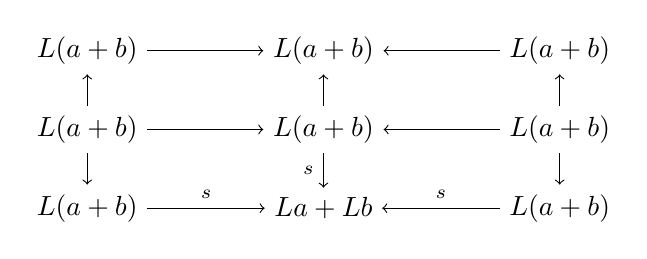
\begin{tikzpicture}
%	\draw [help lines, step=0.5, color=blue!10] (-5,-5) grid (5,5); % grid
	%
	\begin{scope}
	\node (11) at (-3,1) {$ L ( a + b )  $};
	\node (12) at (0,1) {$ L ( a + b )  $};
	\node (13) at (3,1) {$ L ( a + b )  $};
	\node (21) at (-3,0) {$ L ( a + b )  $};
	\node (22) at (0,0) {$ L ( a + b )  $};
	\node (23) at (3,0) {$ L ( a + b )  $};
	\node (31) at (-3,-1) {$ L ( a + b )  $};
	\node (32) at (0,-1) {$ La +  Lb   $};
	\node (33) at (3,-1) {$ L ( a + b )  $};
	\draw [->] (11) to node [] { \scriptsize $  $} (12);
	\draw [->] (13) to node [] { \scriptsize $  $} (12);
	\draw [->] (21) to node [] { \scriptsize $  $} (22);
	\draw [->] (23) to node [] { \scriptsize $  $} (22);
	\draw [->] (31) to node [above] { \scriptsize $ s $} (32);
	\draw [->] (33) to node [above] { \scriptsize $ s $} (32);
	\draw [->] (21) to node [] { \scriptsize $  $} (11);
	\draw [->] (21) to node [] { \scriptsize $  $} (31);
	\draw [->] (22) to node [] { \scriptsize $  $} (12);
	\draw [->] (22) to node [left] { \scriptsize $ s $} (32);
	\draw [->] (23) to node [] { \scriptsize $  $} (13);
	\draw [->] (23) to node [] { \scriptsize $  $} (33);
	\end{scope}
\end{tikzpicture}
\]
%%%%%%%%%%%%%%%%%
%%%%%%%%%%%%%%%%%
\end{document}
